\documentclass[mathserif,10pt]{beamer}

\usepackage{amsfonts}
\usepackage{amsfonts}
\usepackage{amsfonts}
\usepackage{amsmath,amssymb,amsthm,delarray,natbib,graphicx}
\usepackage{amsmath,amssymb,amsthm,natbib,mathtools,graphicx}
\usetheme{Madrid}
\usepackage{beamerthemesplit}
\input FJHDef.tex
\setlength{\parskip}{2ex}
\setlength{\arraycolsep}{0.5ex}
\usepackage{amsmath,amssymb,amsthm,mathtools,bbm,booktabs,array,tikz,pifont,comment,multirow,url,graphicx}

\DeclareMathOperator{\Var}{Var}
\DeclareMathOperator{\INT}{INT}
\DeclareMathOperator{\APP}{APP}
\DeclareMathOperator{\lin}{lin}
\DeclareMathOperator{\up}{up}
\DeclareMathOperator{\lo}{lo}
\DeclareMathOperator{\fix}{fix}
\DeclareMathOperator{\err}{err}
\DeclareMathOperator{\maxcost}{maxcost}
\DeclareMathOperator{\mincost}{mincost}
\newcommand{\herr}{\widehat{\err}}
\newcommand{\Fnorm}[1]{\abs{#1}_{\cf}}
\newcommand{\Ftnorm}[1]{\abs{#1}_{\tcf}}
\newcommand{\Gnorm}[1]{\norm[\cg]{#1}}
\newcommand{\flin}{f_{\text{\rm{lin}}}}

\begin{document}

\newcommand{\R}{\mathbb{R}}
\newtheorem{theo}{Theorem}
\newtheorem{prop}[theorem]{Proposition}
\newtheorem{lem}{Lemma}
\theoremstyle{definition}
\newtheorem{algo}{Algorithm}
\newtheorem{condit}{Condition}
%\newtheorem{assump}{Assumption}
\theoremstyle{remark}
\newtheorem{rem}{Remark}

\newcommand{\sphere}{\mathbb{S}}
%\newcommand{\cc}{\mathcal{C}}
\newcommand{\cq}{\mathcal{Q}}
\newcommand{\bbW}{\mathbb{W}}
%\newcommand{\tP}{\widetilde{P}}
\newcommand{\bg}{{\bf g}}
\newcommand{\bu}{{\bf u}}
\newcommand{\bbu}{\bar{\bf u}}
\newcommand{\bv}{{\bf v}}
\newcommand{\bbv}{\bar{\bf v}}
\newcommand{\bw}{{\bf w}}
\newcommand{\bbw}{\bar{\bf w}}
%\newcommand{\hv}{\hat{v}}



\setlength{\parskip}{2ex}

\beamersetuncovermixins{\opaqueness<1->{0}}{\opaqueness<1->{60}}

\title{Guaranteed, Adaptive, Automatic Algorithms for Univariate Integration: Methods, Cost and Implementation}
\author{Yizhi Zhang}

\institute{Department of Applied Mathematics, Illinois Institute of
Technology }%\\ Chicago, Illinois, USA\\}
\date{ \today}


\frame{\titlepage}

\frame{\frametitle{Contents}
\begin{itemize}

\item Introduction

\item .

\item .

\item .

\item .

\item .

\item .

\item .

\end{itemize}
}


\section{Introduction}

\frame{\frametitle{Motivation}
\begin{itemize}

  \item $\int_{a}^{b}f(x)\text{d}x$

  \item Simple functions such as $\int_{a}^{b}x^2 \text{d}x=x^3/3|_{a}^{b}$. Use pen and paper.

  \item Functions with no analytical solutions such as the standard normal p.d.f $\int_{a}^{b}e^{-x^2/2}/\sqrt{2\pi}\text{d}x$. Use numerical methods.

\end{itemize}
 }


 \frame{\frametitle{Fixed-cost algorithms}
\begin{itemize}
\item The traditional trapezoidal rule and Simpson's rule are typical two examples.

\item   \begin{align}\label{errorsimple}
            \text{err}(f,n)\le\overline{\text{err}}(f,n):=&C(n)\Var(f^{(p)}),
        \end{align}

\item The algorithms provide guarantees when $\Var(f^{(p)})<\sigma$.

\item The algorithms are automatic. Cost $n=C^{-1}(\varepsilon/\sigma)$.

\item The algorithms are not adaptive. The upper bound on variation, $\sigma$ is not dependent on the integrand.

\item A constant $c\cdot f$ may not work.
\end{itemize}
 }

\frame{\frametitle{Adaptive algorithms with no guarantees}
\begin{itemize}
\item MATLAB's {\tt integral} and Chebfun toolbox are typical two examples.

\item The algorithms are adaptive. No $\sigma$ required.

\item The algorithms provide no guarantees.

\item The algorithms can always be fooled by spiky functions.

\end{itemize}

 }


\frame{\frametitle{What do we think of the problem}
\begin{itemize}

  \item The goal is to construct adaptive, automatic algorithms with guarantees of success.

  \item Define the space of integrands in the cone, not ball.

  \item Error bound \eqref{errorsimple} is approximated using only function values.

  \item To fixed-cost algorithms: adaptive, succeed in the cone.

  \item To adaptive algorithms: rigorous proof of how spiky $f$ can be.

\end{itemize}
 }

\frame{\frametitle{Contents}
\begin{itemize}

\item Introduction

\item Problem Statement

\item Data-Driven Error Bounds

\item Multi-step Adaptive Algorithms

\item Lower and Upper Bound on Computational Cost

\item Lower Bound on Complexity

\item Numerical Example

\item Future Work

\end{itemize}
}

\frame{
\begin{center}
\Huge work flow
\end{center}


}


\section{Problem Statement and Assumptions}

\frame{\frametitle{Trapezoidal rule and Simpson's rule}
The composite trapezoidal rule can be defined as:
\begin{equation}\label{traprule}
  T(f,n)=\frac{b-a}{2n}\sum_{j=0}^{n}(f(u_{j})+f(u_{j+1})),
\end{equation}
where
\begin{equation}\label{upts}
u_j=a+\frac{j(b-a)}{n}, \qquad j=0, \ldots, n, \qquad n\in\mathbb{N}.
\end{equation}

The composite Simpson's rule can be defined as:
\begin{equation}\label{simrule}
  S(f,n)=\frac{b-a}{18n}\sum_{j=0}^{3n-1}(f(v_{2j})+4f(v_{2j+1})+f(v_{2j+2})),
\end{equation}
where
\begin{equation}\label{vpts}
v_j=a+\frac{j(b-a)}{6n}, \qquad j=0, \ldots, 6n, \qquad n\in \naturals.
\end{equation}
}


\frame{\frametitle{Error of two methods}
To better define \eqref{errorsimple}:
\begin{align}\label{errorbound}
    \text{err}(f,n)\le\overline{\text{err}}(f,n):=&C(n)\Var(f^{(p)}),\\
    \nonumber&C(n)=
    \begin{cases*}
           \frac{(b-a)^2}{8n^2}, p=1,  & \mbox{trapezoidal rule},\\%\cite[(7.15)]{BraPet11a}, \\
           \frac{(b-a)^4}{93312n^4}, p=3, & \mbox{Simpson's rule}.%\cite[(p.231)]{BraPet11a}.
    \end{cases*}
\end{align}
The error bounds contains the total variation, which is unknown to the users.
}

\frame{\frametitle{Variation and function spaces}
\begin{equation}\label{defvar}
  \Var(f) := \sup \left\{\widehat{V}(f,\{x_i\}_{i=0}^{n+1}), \quad \text{for any }n \in \naturals, \text{ and } \{x_i\}_{i=0}^{n+1}\right\},
\end{equation}
where
\begin{equation}\label{defvhat}
    \widehat{V}(f,\{x_i\}_{i=0}^{n+1})=\sum_{i=1}^{n-1}|f(x_{i+1})-f(x_{i})|.
\end{equation}

To ensure a finite error bound, our algorithms are defined for function spaces with finite total variations of the respective derivatives:
\begin{equation}\label{defspace}
 \cv^{p}:=\{f\in C^{p-1}[a,b]: \Var(f^{(p)}) < \infty \},
\end{equation}
where for the trapezoidal rule, $p=1$, and for the Simpson's rule, $p=3$.
}

\frame{\frametitle{Spaces and subspaces (cones)}
Our algorithms will not work for all $f \in \cv^{p}$ but will work for integrands in cones:
\begin{multline}\label{defcone}
\cc^{p}:=\left\{f\in \cv^{p}, \Var(f^{(p)})\leq \mathfrak{C}(\text{size}(\{x_i\}_{i=0}^{n+1}))\widehat{V}(f^{(p)},\{x_i\}_{i=0}^{n+1}),\right.\\ \left.\text{for all choices of } n\in \mathbb{N}, \text{and }\{x_i\}_{i=0}^{n+1} \text{ with }\text{size}(\{x_i\}_{i=0}^{n+1})<\mathfrak{h}\right\}.
\end{multline}

\begin{equation}\label{defsize}
  \text{size}(\{x_i\}_{i=0}^{n+1}):=\max_{i=0,\cdots, n} x_{i+1}-x_{i}.
\end{equation}

\begin{equation}\label{definflationfactor}
  \mathfrak{C}(h):=\frac{\mathfrak{C}(0)}{1-h/\mathfrak{h}}; \quad \mathfrak{C}(0)>1
\end{equation}

}

\frame{\frametitle{How to find error bounds}
\begin{itemize}
  \item The definition of the cone suggests a way of bounding $\Var(f^{(p)})$ in terms of $\widehat{V}(f^{(p)},\{x_i\}_{i=0}^{n+1})$.
  \item Our algorithms are based on function values and $\widehat{V}(f^{(p)},\{x_i\}_{i=0}^{n+1})$ is defined in terms of derivative values.
  \item Find a way to express derivative values in terms of function values.
\end{itemize}

}

\section{Data-Driven Error Bound}
\frame{\frametitle{Trapezoidal rule}
The backward finite difference is used to approximate $f'$. Let the width of the interval $h=u_{j+1}-u_{j}=(b-a)/n$ and
\begin{align*}
  f[u_{j}]&=f(u_{j}), \text{ for } j=0,\cdots, n,\\
  f[u_{j},u_{j-1}]&=\frac{f(u_{j})-f(u_{j-1})}{h},\text{ for } j=1, \cdots, n.
\end{align*}
According to Mean Value Theorem for finite differences,
\begin{equation}\label{fprime}
  f'(x_j)=\frac{f(u_{j})-f(u_{j-1})}{h}=\frac{n}{b-a}[f(u_{j})-f(u_{j-1})],
\end{equation}
for some $x_j\in (u_{j-1},u_{j})$.
\begin{equation}\label{cutoff1}
  \text{size}(\{x_j\}_{j=0}^{n+1})\leq 2h=2(b-a)/n<\mathfrak{h}.
\end{equation}
}

\frame{\frametitle{Trapezoidal rule, continued}

The approximation $\widetilde{V}_1(f,n)$ to $\widehat{V}(f',\{x_j\}_{i=0}^{n+1})$ using only function values is defined as:
\begin{align}\label{vtilde1}
\nonumber    \widehat{V}(f',\{x_j\}_{j=0}^{n+1})&= \sum_{j=1}^{n-1}\left|f'(x_{j+1})-f'(x_{j})\right|,\\
\nonumber    &=\sum_{j=1}^{n-1}\left|\frac{n}{b-a}[f(u_{j+1})-f(u_{j})-f(u_{j})+f(u_{j-1})]\right|\\
    &=\frac{n}{b-a}\sum_{j=1}^{n-1}\left|f(u_{j+1})-2f(u_{j})+f(u_{j-1})\right|=:\widetilde{V}_1(f,n).
\end{align}
}

\frame{\frametitle{Trapezoidal rule, error bound}
\begin{align*}
\overline{\text{err}}_{\text{t}}(f,n):=&C(n)\Var(f'),\qquad &\text{ (by \eqref{errorbound})}\\
\leq & C(n)\mathfrak{C}(\text{size}(\{x_i\}_{i=0}^{n+1}))\widehat{V}(f',\{x_i\}_{i=0}^{n+1}), \qquad &\text{ (by \eqref{defcone})}\\
=& C(n)\mathfrak{C}(\text{size}(\{x_j\}_{i=0}^{n+1}))\widetilde{V}_1(f,n), \qquad &\text{ (by \eqref{vtilde1})}\\
  \leq & \frac{(b-a)^2\mathfrak{C}(2(b-a)/n)\widetilde{V}_1(f,n)}{8n^2}.\qquad &\text{ (by \eqref{cutoff1})}
\end{align*}


}

\frame{\frametitle{Simpson's rule}
The third order backward finite difference is used to approximate $f'''$. Let $h=v_{j+1}-v_{j}=(b-a)/6n$ be the width of the interval and
\small
\begin{align*}
  f[v_{j}]&=f(v_{j}), &\text{ for } j=0,\cdots, 6n,\\
  f[v_{j},v_{j-1}]&=\frac{f(v_{j})-f(v_{j-1})}{h},&\text{ for } j=1, \cdots, 6n,\\
  f[v_{j},v_{j-1},v_{j-2}]&=\frac{f(v_{j})-2f(v_{j-1})+f(v_{j-2})}{2h^2},&\text{ for } j=2, \cdots, 6n,\\
  f[v_{j},v_{j-1},v_{j-2},v_{j-3}]&=\frac{f(v_{j})-3f(v_{j-1})+3f(v_{j-2})-f(v_{j-3})}{6h^3}, &\text{ for } j=3, \cdots, 6n.
\end{align*}
According to Mean Value Theorem for finite differences,
\begin{align}\label{ftriprime}
  f'''(x_j)==\frac{216n^3}{(b-a)^3}[f(v_{3j})-3f(v_{3j-1})+3f(v_{3j-2})-f(v_{3j-3})].
\end{align}
for some $x_j\in (v_{3j-3},v_{3j})$.
\begin{equation}\label{cutoff3}
    \text{size}(\{x_j\}_{i=0}^{2n+1})\leq 6h=(b-a)/n<\mathfrak{h}.
\end{equation}
}


\frame{\frametitle{Simpson's rule, continued}
The approximation $\widetilde{V}_3(f,n)$ to $\widehat{V}(f''',\{x_i\}_{i=0}^{n+1})$ using only function values can be written as follow:
\begin{align}\label{vtilde3}
\nonumber    \widehat{V}(f''',\{x_j\}_{j=0}^{n+1})&=\sum_{j=1}^{n-1}\left|f'''(x_{j+1})-f'''(x_{j})\right|,\\
\nonumber    &=\sum_{j=1}^{2n-1}\left|\frac{216n}{(b-a)^3}[(f(v_{3j+3})-3f(v_{3j+2})+3f(v_{3j+1})-f(v_{3j}))\right.\\
\nonumber    &\qquad\left.-(f(v_{3j})-3f(v_{3j-1})+3f(v_{3j-2})-f(v_{3j-3}))]\right|\\
\nonumber    &=\frac{216n^3}{(b-a)^3}\sum_{j=1}^{2n-1}\left|f(v_{3j+3})-3f(v_{3j+2})+3f(v_{3j+1})\right.\\
             &\qquad\left.-2f(v_{3j})+3f(v_{3j-1})-3f(v_{3j-2})+f(v_{3j-3})\right|=:\widetilde{V}_3(f,n).
\end{align}
}

\frame{\frametitle{Simpson's rule, error bound}
Therefore the error bound on error estimate for our Simpson's rule algorithm using only function values is obtained as:
\begin{align*}
\overline{\text{err}}_{\text{s}}(f,n):=&C(n)\Var(f'''),\qquad &\text{ (by \eqref{errorbound})}\\
\leq & C(n)\mathfrak{C}(\text{size}(\{x_i\}_{i=0}^{2n+1}))\widehat{V}(f''',\{x_i\}_{i=0}^{2n+1}), \qquad &\text{ (by \eqref{defcone})}\\
=& C(n)\mathfrak{C}(\text{size}(\{x_j\}_{i=0}^{2n+1}))\widetilde{V}_3(f,n), \qquad &\text{ (by \eqref{vtilde3})}\\
  \leq & \frac{(b-a)^4\mathfrak{C}((b-a)/n)\widetilde{V}_3(f,n)}{93312n^4}.\qquad &\text{ (by \eqref{cutoff3})}
\end{align*}
}


\section{Multi-step Adaptive Algorithms}
\frame{\frametitle{Multi-step trapezoidal rule algorithm}

\begin{algo}[Trapezoidal Rule Adaptive Algorithm {\tt integral\_t}] \label{multistagetrapalgo}
Let the sequence of algorithms $\{T_n\}_{n\in \mathbb{N}}$, %$ \widehat{V}(f,\{x_i\}_{i=0}^{n+1})$,
and $\widetilde{V}_1(\cdot,\cdot)$ be as described above.
Let $\mathfrak{h}\le (b-a)$. Set $k=0$, $n_{k}=1$. For any integrand $f$ and error tolerance $\varepsilon$, do the following:
\begin{description}
\item[Step 1. (Re)set the upper bound on $\Var(f')$; increase number of nodes.] Let $\eta_{k}=\infty$ and $n_{k+1}=n_k\times\left\lceil2(b-a)/(\mathfrak{h}n_{k})\right\rceil$.

\item[Step 2. Compute the largest lower bound on {$\Var(f')$}.] Let $k=k+1$. Compute  $\widetilde{V}_1(f,n_k)$ in \eqref{vtilde1}.% and $T_{n_k}(f)$ in \eqref{traprule}.

\item[Step 3. Compute the smallest upper bound on {$\Var(f')$}.] Compute
    \begin{align*}
        \eta_{k}=\min\left(\eta_{k-1},\mathfrak{C}(2(b-a)/n_{k})\widetilde{V}_1(f,n_k)\right).
    \end{align*}
\end{description}
\end{algo}
}


\frame{\frametitle{Multi-step trapezoidal rule algorithm, continued}
\begin{algo}
\begin{description}
\item[Step 4. Check the necessary condition for $f \in \cc^1$.] If $\widetilde{V}_1(f,n_k) \le \eta_{k}$, then go to Step 5.
  Otherwise, set $\mathfrak{h} = \mathfrak{h}/2$.
    \begin{enumerate}
          \item Let $\mathfrak{J}=\{j\in\{1, \cdots, k\}: n_{j}\ge 2(b-a)/\mathfrak{h}\}$. If $\mathfrak{J}$ is empty, go to Step 1.
          \item Otherwise, recompute the upper bound on $\Var(f')$, for all $n_{j}$, with $j \in \mathfrak{J}$ as follows:
          \begin{align*}
           &\text{For } j'=\min\mathfrak{J}, \text{ let } \eta_{j'}=\mathfrak{C}(2(b-a)/n_{j'})\widetilde{V}_1(f,n_{j'}), \\
           &\text{Compute } \\
           &\eta_{j}=\min\{\eta_{j-1},\mathfrak{C}(2(b-a)/n_{j})\widetilde{V}_1(f,n_{j})\}, \text{ for } j=j'+1, \cdots, k.
          \end{align*}
            Go to the beginning of Step 4.
    \end{enumerate}
\end{description}
\end{algo}
}

\frame{\frametitle{Multi-step trapezoidal rule algorithm, continued}
\small
\begin{algo}
\begin{description}
\item[Step 5. Check for convergence.] Check whether $n_k$ is large enough to satisfy the error tolerance, i.e.
    \begin{equation*}
         n_k^2 \ge \frac{\eta_{k}(b-a)^2}{8\varepsilon }.
    \end{equation*}
    \begin{enumerate}
      \item If this is true, return {\tt integral\_t}$(f,\varepsilon)=T_{n_k}(f)$ and terminate the algorithm.
      \item Otherwise, go the Step 6.
    \end{enumerate}

\item[Step 6. Increase the number of nodes and loop again.] Choose
$$
n_{k+1}=n_k\times\max\left(\left\lceil\frac{(b-a)}{n_{k}}\sqrt{\frac{\widetilde{V}_1(f,n_k)}{8\varepsilon}}\right\rceil,2\right).
$$
Go to Step 2.
\end{description}
\end{algo}
}

\frame{\frametitle{Multi-step Simpson's rule algorithm}

\begin{algo}[Simpson's Rule Adaptive Algorithm {\tt integral\_s}] \label{multistageintegalgosimpson}
Let the sequence of algorithms $\{S_n\}_{n\in \mathbb{N}}$, %$ \widehat{V}(f,\{x_i\}_{i=0}^{n+1})$,
and $\widetilde{V}_3(\cdot,\cdot)$ be as described above.
Let $\mathfrak{h}\le (b-a)/6$. Set $k=0$, $n_{k}=0$. For any integrand $f$ and error tolerance $\varepsilon$, do the following: %
\begin{description}
\item[Step 1. (Re)set the upper bound on $\Var(f''')$; increase the number of nodes.] $\quad$ Let $\eta_{k}=\infty$ and $n_{k+1}=n_k\times\left\lceil(b-a)/\mathfrak{h}n_{k}\right\rceil$.

\item[Step 2. Compute the largest lower bound on {$\Var(f''')$}.] Let $k=k+1$. Compute  $\widetilde{V}_3(f,n_k)$ in \eqref{vtilde3}.

\item[Step 3. Compute the smallest upper bound on {$\Var(f''')$}.] Compute
    \begin{align*}
        \eta_{k}=\min\left(\eta_{k-1},\mathfrak{C}((b-a)/n_{k})\widetilde{V}_3(f,n_k)\right).
    \end{align*}
\end{description}
\end{algo}
}


\frame{\frametitle{Multi-step Simpson's rule algorithm, continued}
\begin{algo}
\begin{description}
\item[Step 4. Check the necessary condition for $f \in \cc^3$.] If $\widetilde{V}_3(f,n_k) \le \eta_{k}$, go to Step 5.
  Otherwise, set $\mathfrak{h} = \mathfrak{h}/2$.
    \begin{enumerate}
      \item Let $\mathfrak{J}=\{j\in\{1, \cdots, k: n_{j}\}\ge (b-a)/\mathfrak{h}\}$. If $\mathfrak{J}$ is empty, go to Step 1.
      \item Otherwise, recompute the upper bound on $\Var(f''')$ for all $n_{j}$, with $j \in \mathfrak{J}$ as follows:
      \begin{align*}
        &\text{For } j'=\min\mathfrak{J}, \text{ let } \eta_{j'}=\mathfrak{C}((b-a)/n_{j'})\widetilde{V}_3(f,n_{j'}), \\
        &\text{Compute }\\
        &\eta_{j}=\min\{\eta_{j-1},\mathfrak{C}((b-a)/n_{j})\widetilde{V}_3(f,n_{j})\}, \text{ for } j=j'+1, \cdots, k.
      \end{align*}
      Go to the beginning of Step 4.
    \end{enumerate}
\end{description}
\end{algo}
}

\frame{\frametitle{Multi-step Simpson's rule algorithm, continued}
\small
\begin{algo}
\begin{description}
\item[Step 5. Check for convergence.] Check whether $n_k$ is large enough to satisfy the error tolerance, i.e.

    \begin{equation*}
          n_k^4 \ge \frac{\eta_{k}(b-a)^4}{93312\varepsilon}.
    \end{equation*}

    \begin{enumerate}
      \item If true, return {\tt integral\_s}$(f,\varepsilon)=S_{n_k}(f)$ and terminate the algorithm.
      \item Otherwise, go the Step 6.
    \end{enumerate}

\item[Step 6. Increase the number of nodes and loop again.] Choose
$$
n_{k+1}=n_k\times\max\left(\left\lceil\frac{(b-a)}{n_{k}}\left(\frac{\widetilde{V}_3(f,n_k)}{93312\varepsilon}\right)^{1/4}\right\rceil,2\right).
$$
Go to Step 2.
\end{description}
\end{algo}
}




\section{Lower and Upper Bound on Computational Cost}
\frame{\frametitle{Computational cost of the trapezoidal rule}
\small
\begin{theorem}\label{uppbndcost}
     Let $N(f,\varepsilon)$ denote the final number $n_k$ in Step 5 when {\tt integral\_t} terminates. Then this number is bounded below and above in terms of the true, yet unknown, $\Var(f')$.
    \begin{multline}\label{uppbndcosttrapineq}
        \max\left(\left\lfloor\frac{2(b-a)}{\mathfrak{h}}\right\rfloor,\left\lceil2(b-a)\sqrt{\frac{\Var(f')}{8\varepsilon}}\right\rceil\right)\leq N(f,\varepsilon)\\ \leq 2\min\left\{n\in\mathbb{N}:n\geq\left(\left\lfloor\frac{2(b-a)}{\mathfrak{h}}\right\rfloor\right),\zeta(n)\Var(f')\leq\varepsilon\right\}\\ \leq 2\min_{0<\alpha\leq1}\max\left(\left(\left\lfloor\frac{2(b-a)}{\alpha\mathfrak{h}}\right\rfloor\right),(b-a)\sqrt{\frac{\mathfrak{C}(\alpha\mathfrak{h})\Var(f')}{8\varepsilon}}\right),
    \end{multline}
    where $\zeta(n)=(b-a)^2\mathfrak{C}(2(b-a)/n)/(8\varepsilon n^2)$. The number of function values, namely, the computational cost required by the algorithm, is $N(f,\varepsilon)+1$.
\end{theorem}
}

\frame{\frametitle{Computational cost of the Simpson's rule}
\small
\begin{theorem}\label{uppbndcostSimp}
    Let $N(f,\varepsilon)$ denote the final number of $n_k$ in Step 5 when {\tt integral\_s} terminates. Then this number is bounded below and above in terms of the true, yet unknown, $\Var(f''')$.
    \begin{multline}\label{uppbndcostineqsim}
        \max\left(\left\lfloor\frac{(b-a)}{\mathfrak{h}}\right\rfloor,\left\lceil(b-a)\left(\frac{\Var(f''')}{93312\varepsilon}\right)^{1/4}\right\rceil\right)\leq N(f,\varepsilon)\\ \leq 2\min\left\{n\in\mathbb{N}:n\geq\left(\left\lfloor\frac{(b-a)}{\mathfrak{h}}\right\rfloor\right),\zeta(n)\Var(f''')\leq\varepsilon\right\}\\ \leq 2\min_{0<\alpha\leq1}\max\left(\left(\left\lfloor\frac{(b-a)}{\alpha\mathfrak{h}}\right\rfloor\right),(b-a)\left(\frac{\mathfrak{C}(\alpha\mathfrak{h})\Var(f''')}{93312\varepsilon}\right)^{1/4}\right),
    \end{multline}
    where $\zeta(n)=(b-a)^4\mathfrak{C}((b-a)/n)/(93312n^4)$. The number of function values, namely the computational cost, required by the algorithm is $6N(f,\varepsilon)+1$.
\end{theorem}
}

\frame{\frametitle{Computational cost of the Simpson's rule, continued}
\begin{proof}\renewcommand{\qedsymbol}{}
  No matter what inputs $f$ and $\varepsilon$ are provided, $N(f,\varepsilon)\ge n_1=\lfloor (b-a)/\mathfrak{h}\rfloor$. Then the number of intervals increases until $\overline{\text{err}}(f,n)\le\varepsilon$. From the error bound defined in \eqref{errorbound}, $C(N(f,\varepsilon))\Var(f''')\leq \varepsilon$. Thus $N(f,\varepsilon)\geq \left\lceil(b-a)\left(\frac{\Var(f''')}{93312\varepsilon}\right)^{1/4}\right\rceil$. This implies the lower bound on $N(f,\varepsilon)$.
\end{proof}
}

\frame{\frametitle{Computational cost of the Simpson's rule, continued}
\begin{proof}\renewcommand{\qedsymbol}{}
 Let $K$ be the value of $k$ for which {\tt integral\_s} terminates. Since $n_1$ satisfies the upper bound, one may assume that $K \ge 2$. Let $m$ be the multiplication integer found in Step 6. Note that $\zeta((m-1)n_{K-1})\Var(f''')>\varepsilon$. For $m=2$, this is true because $\zeta(n_{K-1})\Var(f''')\ge\zeta(n_{K-1})\widetilde{V}_{3}(f,n_{K-1})>\varepsilon$. For $m>2$ it is true because of the definition of $m$. Since $\zeta$ is a decreasing function, it follows that
  $$(m-1)n_{K-1}<n^*:=\min\left\{n\in\mathbb{N}:n\ge\left\lfloor\frac{2(b-a)}{n}\right\rfloor,\zeta(n)\Var(f''')\le\varepsilon\right\}.$$
  Therefore $n_K=m^*n_{K-1}<m^*\frac{n^*}{m-1}=\frac{m}{m-1}n^*\le2n^*$.
  \end{proof}
}

\frame{\frametitle{Computational cost of the Simpson's rule, continued}
\footnotesize
\begin{proof}%\renewcommand{\qedsymbol}{}
  For fixed $\alpha\in(0,1]$, we only need to consider that case where $n^*>\left\lfloor2(b-a)/(\alpha\mathfrak{h})\right\rfloor$. This implies that $n^*>\left\lfloor2(b-a)/(\alpha\mathfrak{h})\right\rfloor\ge 2(b-a)/(\alpha\mathfrak{h})$ thus $\alpha\mathfrak{h}\ge2(b-a)/(n^*)$. Also by the definition of $n^*$, $\zeta$, and $\mathfrak{C}$ is non-decreasing:
  \begin{align*}
    &\zeta(n^*)\Var(f''')>\varepsilon, \\
    \Rightarrow 1&<\left(\frac{\zeta(n^*)\Var(f''')}{\varepsilon}\right)^{1/4},\\
    \Rightarrow n^*&<n^*\left(\frac{\zeta(n^*)\Var(f''')}{\varepsilon}\right)^{1/4},\\
    &=n^*\left(\frac{(b-a)^4\mathfrak{C}(2(b-a)/(n^*))\Var(f''')}{93312(n^*)^4\varepsilon}\right)^{1/4},\\
    &\le(b-a)\left(\frac{\mathfrak{C}(\alpha\mathfrak{h})\Var(f''')}{93312\varepsilon}\right)^{1/4}.
  \end{align*}
  \end{proof}
}

\section{Lower Bound on Complexity}
\frame{\frametitle{Lower bound on complexity for the Simpson's rule}
Use
 \begin{align} \label{bumpfunction}
\text{bump}(x;t,h):= \begin{cases} \displaystyle (x-t)^3/6,  &t \le x < t+\delta,\\[1ex]
\displaystyle [-3(x-t)^3+12\delta(x-t)^2\\[1ex] \displaystyle\qquad -12\delta^2(x-t)+4\delta^3]/6,  &t+\delta \le x < t+2\delta,\\[1ex]
\displaystyle [3(x-t)^3-24\delta(x-t)^2\\[1ex]  \displaystyle\qquad +60\delta^2(x-t)-44\delta^3]/6, &t+2\delta \le x < t+3\delta,\\[1ex]
\displaystyle (t+4\delta-x)^3/6,  &t+3\delta \le x < t+4\delta,\\[1ex]
\displaystyle  0,  &\text{otherwise},
\end{cases}
\end{align}

}


\frame{
to build the fooling function
\begin{equation*}
        \text{twobp}(x;t,\delta,\pm):=\text{bump}(x;a,\mathfrak{h})\pm\frac{15[\mathfrak{C}(\delta)-1]}{16}\text{bump}(x;t,\delta)
\end{equation*}

Although $\text{twobp}'''(x;t,\delta,\pm)$ may have a bump with arbitrarily small width $4\delta$, the height is small enough for $\text{twobp}'''(x;t,\delta,\pm)$ to lie in the cone.
}


\frame{\frametitle{Lower bound on complexity for the trapezoidal rule}
\begin{figure}[ht]
\centering
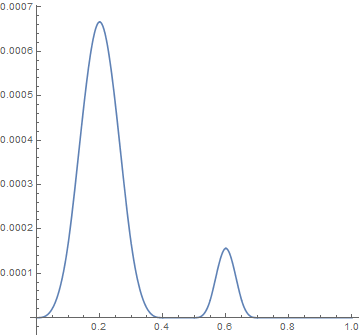
\includegraphics[width=5.5cm]{twobp.png}
\caption{A fooling function that can fool the Simpson's rule algorithms, where $a=0$, $b=1$, $t=0.5$, $\delta=0.05$ and $\mathfrak{h}=0.1$. \label{fig:twobpfunction}}
\end{figure}


}




\frame{\frametitle{Lower bound on the complexity for the Simpson's rule}

\begin{theorem}\label{compsim}
    Let $\texttt{int}$ be any (possibly adaptive) algorithm that succeeds for all integrands in $\cc^3$, and only uses integrand values. For any error tolerance $\varepsilon > 0$ and any arbitrary value of $\Var(f''')$, there will be some $f\in \cc^3$ for which $\texttt{int}$ must use at least
    \begin{equation}\label{complowbdsim}
        -\frac{5}{4}+\frac{b-a-5\mathfrak{h}}{8}\left[\frac{[\mathfrak{C}(0)-1]\Var( f''')}{\varepsilon}\right]^{1/4}
    \end{equation}
    function values. As $\Var(f''')/\varepsilon \rightarrow \infty$ the asymptotic rate of increase is the same as the computational cost of {\tt integral\_s}. Thus {\tt integral\_s} has optimal order for integration of functions in $\cc^3$.
\end{theorem}

}

\frame{\frametitle{Lower bound on the complexity for the Simpson's rule, continued}

\begin{proof}\renewcommand{\qedsymbol}{}
  For any positive $\alpha$, suppose that $\texttt{int}(\cdot,\varepsilon)$ evaluates integrand $\alpha\text{bump}'''(\cdot;t,\delta)$ at $n$ nodes before returning to an answer. Let $\{x_j\}_{j=1}^{m})$ be the $m<n$ ordered nodes used by $\texttt{int}(\cdot,\varepsilon)$ that fall in the interval $(x_{0},x_{m+1})$ where $x_{0}:=a+3\mathfrak{h}$, $x_{m+1}:=b-\delta$ and $\delta:=(b-a-5\mathfrak{h})/(4n+5)$. There must exits at least one of these $x_{j}$ with $i=0,\cdots,m$ for which
  \begin{align*}
    \frac{x_{j+1}-x_{j}}{4}\ge\frac{x_{m+1}-x_{0}}{4(m+1)}\ge\frac{x_{m+1}-x_{0}}{4(n+1)}=\frac{b-a-5\mathfrak{h}-\delta}{4n+4}=\delta.
  \end{align*}
  
\end{proof}

}

\frame{\frametitle{Lower bound on the complexity for the Simpson's rule, continued}

\begin{proof}\renewcommand{\qedsymbol}{}
  
  Choose one such $x_{j}$ and call it $t$. The choice of $t$ and $\delta$ ensures that $\texttt{int}(\cdot,\varepsilon)$ cannot distinguish between $\alpha\text{bump}(\cdot;t,\delta)$ and $\alpha\text{twobp}(\cdot;t,\delta,\pm)$. Thus
  \begin{align*}
    \texttt{int}(\alpha\text{twobp}(\cdot;t,\delta,\pm),\varepsilon)=\texttt{int}(\alpha\text{bump}(\cdot;t,\delta),\varepsilon)
  \end{align*}
  Moreover, $\alpha\textup{bump}(\cdot;t,\delta)$ and $\alpha\textup{twobp}(\cdot;t,\delta,\pm)$ are all in the cone $\cc^3$. This means that $\texttt{int}(\cdot,\varepsilon)$ is successful for all of the functions.
  
\end{proof}

}

\frame{\frametitle{Lower bound on the complexity for the Simpson's rule, continued}

\begin{proof}\renewcommand{\qedsymbol}{}
\tiny
  \begin{subequations}
  \begin{multline*}
    \varepsilon\ge\frac{1}{2}\left[\right.\left|\int_{a}^{b}\alpha\textup{twobp}(x;t,\delta,-)dx-\texttt{int}(\alpha\textup{twobp}(\cdot;t,\delta,-),\varepsilon)\right|\\
    +\left|\int_{a}^{b}\alpha\textup{twobp}(x;t,\delta,+)dx-\texttt{int}(\alpha\textup{twobp}(\cdot;t,\delta,+),\varepsilon)\right|\left.\right]
  \end{multline*}
  \begin{align*}
     &\ge\frac{1}{2}\left|\int_{a}^{b}\alpha\textup{twobp}(x;t,\delta,+)dx-\int_{a}^{b}\alpha\textup{twobp}(x;t,\delta,-)dx\right|\\
     &=\int_{a}^{b}\alpha\textup{bump}(x;t,\delta)dx\\
     &=\frac{15\alpha[\mathfrak{C}(\delta)-1]\delta^4}{16}\\
     &=\frac{[\mathfrak{C}(\delta)-1]\delta^4\Var(\alpha\textup{bump}'''(\cdot;a,\mathfrak{h}))}{16}
  \end{align*}
  \end{subequations}
\end{proof}

}

\frame{\frametitle{Lower bound on the complexity for the Simpson's rule, continued}

\begin{proof}
 
  Substituting $\delta$  in terms of $n$:
      \begin{align*}
        4n+5=\frac{b-a-5\mathfrak{h}}{\delta}&\ge(b-a-5\mathfrak{h})\left[\frac{[\mathfrak{C}(\delta)-1]\Var(\alpha \textup{bump}'''(\cdot;a,\mathfrak{h})))}{16\varepsilon}\right]^{1/4},\\
        &\ge-\frac{5}{4}+\frac{b-a-5\mathfrak{h}}{8}\left[\frac{[\mathfrak{C}(0)-1]\Var(\alpha \textup{bump}'''(\cdot;a,\mathfrak{h}))}{\varepsilon}\right]^{1/4}.
    \end{align*}
    Since $\alpha$ is an arbitrary positive number, the value of $\Var(\alpha \texttt{bump}'''(\cdot;a,\mathfrak{h}))$ is arbitrary.

    Finally, {\tt integral\_s} is optimal.
\end{proof}

}


\section{Numerical Example}

\frame{\frametitle{Numerical Example}
The bump function $\text{bump}(x;t,\delta)$ defined in \eqref{bumpfunction} is used as our test function to check the performance of our algorithms. Consider the family of bump test functions on interval $(0,1)$ defined by
\begin{equation}\label{testfun}
f(x,t,\delta)= \text{bump}(x;t,\delta)/\delta^{4}
\end{equation}
with  $t \sim \cu[0,1-4\delta]$, $\log_{10}(\delta) \sim \cu[-4,-1]$. The integration $\int_{0}^{1}f(x,t,\delta)\text{d}x=1$.
}

\frame{\frametitle{Experiment Setup}


As an experiment, we chose $10000$ random test functions and applied {\tt integral\_t} and {\tt integral\_s} with an error tolerance of  $\varepsilon = 10^{-8}$. The initial values of $\mathfrak{h}$ are set as $0.1$, $0.01$, and $0.001$. The algorithm is considered successful for a particular $f$ if the exact and approximate integrals have a difference no greater than $\varepsilon$. Our algorithms give warnings when the integrand is not in the original cone.

Some commonly available numerical algorithms in MATLAB are {\tt integral}  and the Chebfun toolbox. We applied these two routines to the random family of test functions as well.  Their success and failure rates are also recorded in Table \ref{integresultstable}.  They do not give warnings of possible failure.
}

\frame{\frametitle{Results}
\begin{table}[ht]
\caption{The success rates of {\tt integral\_t} and {\tt integral\_s} plus the success rates of other common quadrature algorithms.}
\centering
\begin{tabular}{cccc}
\hline\hline
& $\mathfrak{h}$ & Success & Success Warning \\
\hline
&$0.1$  & $24.76\%$ &  $9.43\%$  \\
{\tt integral\_t}
 &$0.01$  & $57.36\%$ & $3.70\%$ \\
&$0.001$ & $87.38\%$ &$0.81\%$ \\
\hline
&$0.1$  & $25.94\%$ &  $14.28\%$  \\
{\tt integral\_s}
 &$0.01$  & $57.63\%$ & $4.45\%$ \\
&$0.001$ & $94.09\%$ &$0.87\%$ \\
\hline
{\tt integral} & & 29.68 \% & \\
{\tt chebfun} & &18.91\% & \\
\hline
\end{tabular}
\label{integresultstable}
\end{table}
}

\frame{\frametitle{Convergence rates}
The test function is $f(x,t,\delta)= \text{bump}(x;t,\delta)/\delta^{4}$ where $t=0.2$; $\delta=0.1$. Both {\tt integral\_t} and {\tt integral\_s} use $\mathfrak{h}=0.1$.
\begin{figure}[ht]
\centering
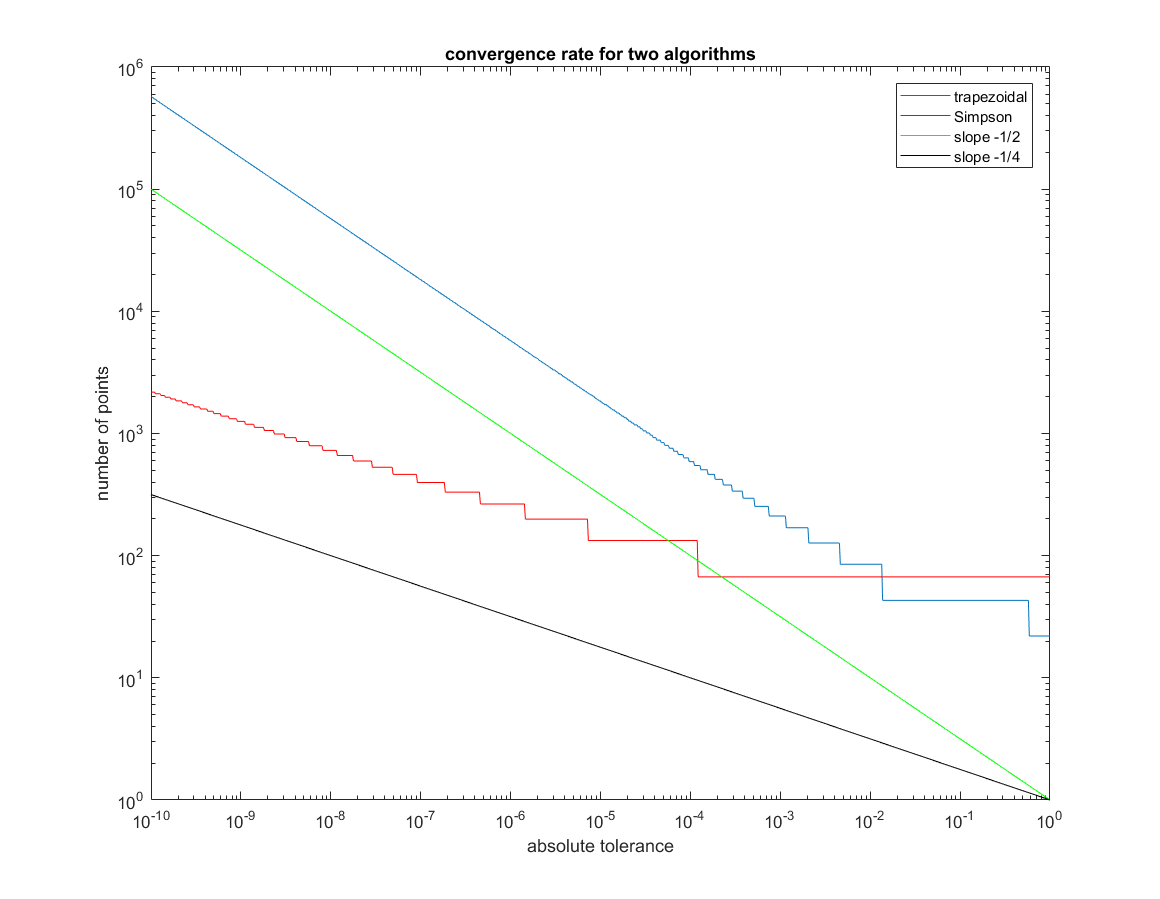
\includegraphics[width=5.5cm]{converwithslope.png}
\caption{The convergence curves for {\tt integral\_t} and {\tt integral\_s}. \label{fig:convergencerate}}
\end{figure}
}
%\frame{\frametitle{Guaranteed Automatic Integration Library (GAIL)}
%
%The ideas presented here are being implemented in MATLAB code (code.google.com$\backslash$p$\backslash$gail), which also include:
% \begin{itemize}
%
%   \item Automatic univariate function recovery via linear splines.
%
%   \item Guaranteed automatic Monte Carlo algorithm for multidimensional integration.
%
%   \item Guaranteed automatic quasi-Monte Carlo algorithm for multidimensional integration.
%
%   \item And more.
% \end{itemize}
%}

%\frame{\frametitle{Summary}
% \begin{itemize}
%   \item  Most popular algorithms are not automatic. Those that are automatic are not guaranteed. We need to request them or build them.
%
%
%   \item Think cones, not balls.
% \end{itemize}
%
%}

\section{Future Work}
\frame{\frametitle{Future Work}
 \begin{itemize}

%   \item Extend the integral from $[0,1]$ to $[a,b]$.

   \item Guaranteed automatic algorithms with higher order convergence rate.

   \item Locally adaptive algorithms.

   \item Relative Error.

 \end{itemize}
}


\frame{
\begin{center}
\Huge Thank you!
\end{center}


}

\frame{\frametitle{how to find the inflation number}
We hope the number of points for the next loop to be large enough such that
$$
n^{4}_{k+1}\ge\frac{(b-a)^4\Var(f''')}{93312\varepsilon}.
$$
Underestimate $\Var(f''')$ with $\widetilde{V}_{1}(f,n_k)$.
}

\frame{\frametitle{how to find the quarter length}
The average width of intervals is $(x_{m+1}-x_{0})/(m+1)$ and $x_{m+1}-x_{0}=b-a-5\mathfrak{h}-\delta$. Choose one interval such that width less bigger than $4\delta$ . We can choose interval wider than average and $4\delta$ narrower than average:
  \begin{align*}
    \frac{x_{j+1}-x_{j}}{4}&\ge\frac{x_{m+1}-x_{0}}{4(m+1)}\ge\frac{x_{m+1}-x_{0}}{4(n+1)}=\frac{b-a-5\mathfrak{h}-\delta}{4n+4}=\delta,\\
    \Rightarrow \delta&=\frac{b-a-5\mathfrak{h}}{4n+5}
  \end{align*}
}

%\frame{\frametitle{References 1}
%
%Clancy N, Ding Y, Hamilton C, Hickernell FJ, Zhang Y (2013) The complexity of guaranteed automatic algorithms: Cones, not balls. Submitted for publication, arXiv.org:1303.2412 [math.NA]
%}

\frame{\frametitle{Computational cost of the trapezoidal rule}
\small
\begin{theorem}\label{uppbndcost}
     Let $N(f,\varepsilon)$ denote the final number $n_k$ in Step 5 when {\tt integral\_t} terminates. Then this number is bounded below and above in terms of the true, yet unknown, $\Var(f')$.
    \begin{multline}\label{uppbndcosttrapineq}
        \max\left(\left\lfloor\frac{2(b-a)}{\mathfrak{h}}\right\rfloor,\left\lceil2(b-a)\sqrt{\frac{\Var(f')}{8\varepsilon}}\right\rceil\right)\leq N(f,\varepsilon)\\ \leq 2\min\left\{n\in\mathbb{N}:n\geq\left(\left\lfloor\frac{2(b-a)}{\mathfrak{h}}\right\rfloor\right),\zeta(n)\Var(f')\leq\varepsilon\right\}\\ \leq 2\min_{0<\alpha\leq1}\max\left(\left(\left\lfloor\frac{2(b-a)}{\alpha\mathfrak{h}}\right\rfloor\right),(b-a)\sqrt{\frac{\mathfrak{C}(\alpha\mathfrak{h})\Var(f')}{8\varepsilon}}\right),
    \end{multline}
    where $\zeta(n)=(b-a)^2\mathfrak{C}(2(b-a)/n)/(8\varepsilon n^2)$. The number of function values, namely, the computational cost required by the algorithm, is $N(f,\varepsilon)+1$.
\end{theorem}
}


\frame{\frametitle{Computational cost of the trapezoidal rule, continued}
\begin{proof}\renewcommand{\qedsymbol}{}
 No matter what inputs $f$ and $\varepsilon$ are provided, $N(f,\varepsilon)\ge n_1=\lfloor 2(b-a)/\mathfrak{h}\rfloor$. Then the number of intervals increases until $\overline{\text{err}}(f,n)\le\varepsilon$. From the error bound defined in \eqref{errorbound}, $C(N(f,\varepsilon))\Var(f')\leq \varepsilon$. Thus $N(f,\varepsilon)\geq \left\lceil2(b-a)\sqrt{\Var(f')/(8\varepsilon)}\right\rceil$. This implies the lower bound on $N(f,\varepsilon)$.
\end{proof}
}

\frame{\frametitle{Computational cost of the trapezoidal rule, continued}
\begin{proof}\renewcommand{\qedsymbol}{}
 Let $K$ be the value of $k$ for which {\tt integral\_t} terminates. Since $n_1=\left\lfloor2(b-a)/\mathfrak{h}\right\rfloor$ satisfies the upper bound, one may assume that $K \ge 2$. Let $m$ be the multiplication integer found in Step 6. Note that $\zeta((m-1)n_{K-1})\Var(f')>\varepsilon$. For $m=2$, this is true because $\zeta(n_{K-1})\Var(f')\ge\zeta(n_{K-1})\widetilde{V}_{1}(f,n_{K-1})>\varepsilon$. For $m>2$ it is true because of the definition of $m$. Since $\zeta$ is a decreasing function, it follows that
  $$(m-1)n_{K-1}<n^*:=\min\left\{n\in\mathbb{N}:n\ge\left\lfloor\frac{2(b-a)}{n}\right\rfloor,\zeta(n)\Var(f')\le\varepsilon\right\}.$$
  Therefore $n_L=mn_{L-1}<m\frac{n^*}{m-1}=\frac{m}{m-1}n^*\le2n^*$.
  \end{proof}
}

\frame{\frametitle{Computational cost of the trapezoidal rule, continued}
\footnotesize
\begin{proof}%\renewcommand{\qedsymbol}{}
   For fixed $\alpha\in(0,1]$, we only need to consider that case where $n^*>\left\lfloor2(b-a)/(\alpha\mathfrak{h})\right\rfloor$. This implies that $n^*>\left\lfloor2(b-a)/(\alpha\mathfrak{h})\right\rfloor\ge 2(b-a)/(\alpha\mathfrak{h})$ thus $\alpha\mathfrak{h}\ge2(b-a)/n^*$. Also by the definition of $n^*$, $\zeta$, and $\mathfrak{C}$ is non-decreasing:
  \begin{align*}
    &\zeta(n^*)\Var(f')>\varepsilon, \\
    \Rightarrow 1&<\left(\frac{\zeta(n^*)\Var(f')}{\varepsilon}\right)^{1/2},\\
    \Rightarrow n^*&<n^*\left(\frac{\zeta(n^*-1)\Var(f')}{\varepsilon}\right)^{1/2},\\
    &=n^*\left(\frac{(b-a)^2\mathfrak{C}(2(b-a)/n^*)\Var(f')}{8(n^*)^2\varepsilon}\right)^{1/2},\\
    &\le(b-a)\sqrt{\frac{\mathfrak{C}(\alpha\mathfrak{h})\Var(f')}{8\varepsilon}}.
  \end{align*}
  \end{proof}
}

%\frame{\frametitle{Lower bound on complexity for the trapezoidal rule}
% Now we compute the lower bound by constructing fooling functions. We choose  the triangle shaped function $f_0: x \mapsto 1/2-\abs{1/2-x}$. Then
%\begin{gather*}
%\Ftnorm{f_0}=\norm[1]{f'_0-f_0(1)+f_0(0)}=\int_0^1 \abs{\sign(1/2-x)} \, \dif x = 1, \\ \Fnorm{f_0}=\Var(f'_0)=2= \tau_{\min}.
%\end{gather*}
%
%}

%\frame{\frametitle{Lower bound on complexity for the trapezoidal rule, continued}
% For any $n \in \cj:=\natzero$, suppose that the one has the data $L_i(f)=f(\xi_i)$, $i=1, \ldots, n$ for arbitrary $\xi_i$, where $0=\xi_0 \le \xi_1 < \cdots < \xi_n \le \xi_{n+1} = 1$.  There must be some $j=0, \ldots, n$ such that $\xi_{j+1} - \xi_j \ge 1/(n+1)$.  The function $f_{1}$ is defined as a triangle function on the interval $[\xi_j, \xi_{j+1}]$:
%$$
%f_{1}(x):=\begin{cases} \displaystyle
%\frac{\xi_{j+1}-\xi_{j}-\abs{\xi_{j+1}+\xi_{j}-2x}}{8} & \xi_{j} \le x \leq \xi_{j+1},\\
%0 & \text{otherwise}.
%\end{cases}
%$$
%}
%
%\frame{\frametitle{Lower bound on complexity for the trapezoidal rule, continued}
%This is a piecewise linear function whose derivative changes from $0$ to $1/4$ to $-1/4$ to $0$ provided $0 < \xi_j < \xi_{j+1} < 1$, and so $\Fnorm{f_1}=\Var(f'_1)\le 1$. Moreover,
%\begin{gather*}
%\INT(f)=\int_0^1 f_1(x) \, \dif x = \frac{(\xi_{j+1} - \xi_j)^2}{16} \ge \frac{1}{16(n+1)^2} =: g(n),\\
%g^{-1}(\varepsilon)=\left \lceil \sqrt{\frac{1}{16 \varepsilon}} \right \rceil - 1.
%\end{gather*}
%Using these choices of $f_0$ and $f_1$, along with the corresponding $g$ above, we can have that the complexity of the integration problem over the cone of functions $\cc_{\tau}$ is bounded below as
%\begin{equation*}
%\comp(\varepsilon,\ca(\cc_{\tau},\reals,\INT,\Lambda^{\std}),\cb_{s}) \ge \left \lceil \sqrt{\frac{(\tau-2)s}{32 \tau \varepsilon}} \right \rceil -1 .
%\end{equation*}
%
%}


\end{document}



